\documentclass{article}
\usepackage[utf8]{inputenc}
\usepackage[T1]{fontenc}
\usepackage[english]{babel}
\usepackage{fullpage}
\usepackage{color}
\usepackage[table]{xcolor}
\usepackage{listings}
\usepackage{amssymb}
 \def \de {{\rm d}}
\definecolor{darkWhite}{rgb}{0.94,0.94,0.94}
 \usepackage[cache=false]{minted}
\definecolor{LightGray}{gray}{0.9}
\definecolor{monOrange}{rgb}{0.97,0.35,0.04}
\usepackage{tikz}

\newcommand{\mybox}[1]{\fbox{$\displaystyle#1$}}
\newcommand{\myredbox}[1]{\fcolorbox{red}{white}{$\displaystyle#1$}}
\newcommand{\mydoublebox}[1]{\fbox{\fbox{$\displaystyle#1$}}}
\newcommand{\myreddoublebox}[1]{\fcolorbox{red}{white}{\fcolorbox{red}{white}{$\displaystyle#1$}}}
%%%%%%%%%%%%%%%%%%%
\title{Méthode des éléments finis: TD2}
\author{Ibrahim ALAME}
\date{14/02/2024}
\begin{document}
\maketitle
\subsubsection*{Problème de poutre simple}
Une barre est une poutre qui ne transmet que des efforts de traction compression à ses extrémités. On considère une barre $OL$ homogène de module $E$, section constante $A$ et de longueur $L$ soumise à une sollicitation linéïque  $p(x)$ et à deux forces aux extrémités $\vec{f}_1$ et $\vec{f}_2$. Les équations du problème sont les suivantes:
\[
({\cal P}_0)\;\left\{
\begin{array}{lcr}
\displaystyle \frac{\de N}{\de x}+p(x)=0;&0\leq x\leq L &\mbox{ équation d'équilibre } \\
N=EA\displaystyle \frac{\de u}{dx}& 0\leq x\leq L&\mbox{ loi de comportement } \\
N(0)=-f_0 ;N(L)=f_L&&\quad\mbox{ conditions aux limites } 
\end{array}
\right.
\]
où $N(x)$ est l'effort normale à la section transversale d'abscisse $x$ et $u(x)$ est l'allongement en $x$, $u_1$ et $u_2$ sont les déplacements aux extrémités $0$ et $L$. $f_1$ et $f_2$ sont des des forces appliquées en $0$ et $L$.
\begin{center}
 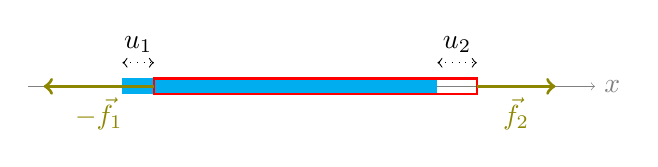
\begin{tikzpicture}[scale=1]
\draw  [very thin, gray] [->]  (-0.2,0) -- (7,0) node[right] {$x$};
\draw (1.2,0.3) node[above] {$u_1$};
\draw (5.25,0.3) node[above] {$u_2$};
\fill[cyan] (1,-0.1) rectangle (5,0.1);
\draw[red,thick=2] (1.4,-0.1) rectangle (5.5,0.1);
\draw[dotted,<->] (1,0.3) -- (1.4,0.3);
\draw[dotted,<->] (5,0.3) -- (5.5,0.3);
\draw[very thick,olive,<-] (0,0) -- (1.4,0) node[below, midway]{$-\vec{f_1}$};
\draw[very thick,olive,->] (5.5,0) -- (6.5,0) node[below, midway]{$\vec{f_2}$};
%\draw [domain=0:5][line width=1] plot(\x,{.8598e-1*\x*\x*\x-.8104*\x*\x+1.697*\x});
%\draw [domain=0:6] plot(\x,{sin(57.29*\x)});
\end{tikzpicture} 
\end{center}

\begin{enumerate}
\item Montrer que le problème $({\cal P}_0)$ se ramène au problème  $({\cal P})$ suivant:
\[
({\cal P})\;\left\{
\begin{array}{l}
-\displaystyle EA\frac{\de^2 u}{dx^2}=p\quad \mbox{dans } ]0,L[\\
 EA\frac{\de u}{dx}(0)=-f_0 \mbox{ , } EA\frac{\de u}{dx}(L)=f_L
\end{array}
\right.
\]
\item Soit $V=H^1(\Omega)$. Montrer que la formulation variationnelle s'écrit comme un problème abstrait de la forme:
\[
({\cal P}_v)\;\left\{
\begin{array}{l}
\mbox{Trouver } u\in V \mbox{ vérifiant}\\
a(u,v)=\ell(v)\quad \forall v\in V
\end{array}
\right.
\]
où \[ a(u,v)=\displaystyle EA\int_0^L\frac{\de u}{dx}\cdot \frac{\de v}{dx}\,\de x\]
et \[ \ell(v)=\displaystyle \int_0^L p\cdot v(x)\de x+f_0 \cdot v(0)+f_L \cdot v(L)\]
\item On fait un maillage en $n+1$ points équidistants. L'élément fini $K$ est un segment de type (1) de longueur $h=\frac 1n$, l'espace de polynômes d'interpolation est $\mathbb{P}_1=\{ax+b,\;(a,b)\in \mathbb{R}^2\}$. les deux fonctions de base $\varphi_1=\lambda_1=1-\frac{x}{h}$ et $\varphi_2=\lambda_2=\frac{x}{h}$.  Calculer $(a(\varphi_i,\varphi_j))_{ij}$ et montrer que le système élémentaire s'écrit:
\[\myredbox{\frac{EA}{h}\left(\begin{array}{rr} 
1&-1\\-1&1
\end{array}\right) \left(\begin{array}{l} 
u_{1}\\u_{2}
\end{array}\right)=\left(\begin{array}{r} 
f_{1}\\f_{2}
\end{array}\right)}
\]
\end{enumerate}
\subsubsection*{Cas d'une poutre à section variable}
On considère la poutre à section variable suivante:
\begin{center}
 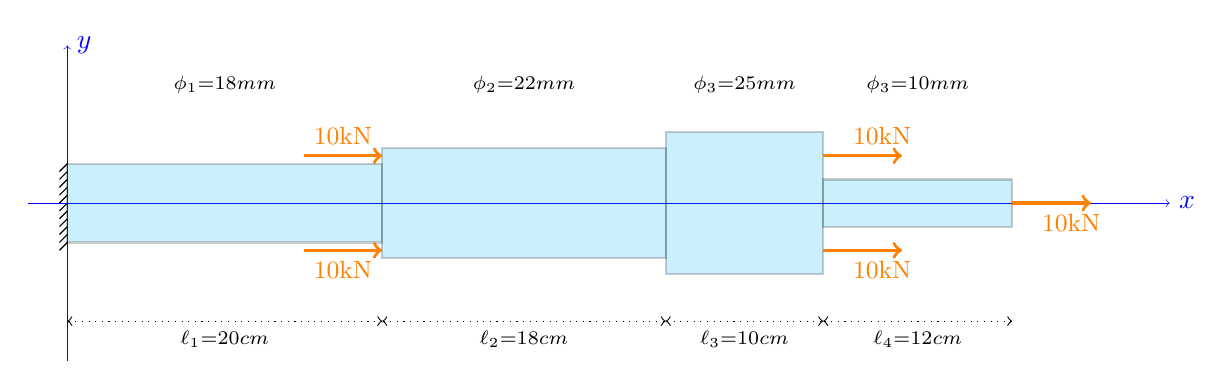
\begin{tikzpicture}[scale=1]
\draw  [very thin, blue] [->]  (-0.5,0) -- (14,0) node[right] {$x$};
\draw  [very thin, blue] [->]  (0,-2) -- (0,2) node[right] {$y$};
\draw[fill=cyan,thick=2, opacity=0.2] (0,-0.5) rectangle (4,0.5);
\draw[fill=cyan,thick=2, opacity=0.2] (4,-0.7) rectangle (7.6,0.7);
\draw[fill=cyan,thick=2, opacity=0.2](7.6,-0.9) rectangle (9.6,0.9);
\draw[fill=cyan,thick=2, opacity=0.2](9.6,-0.3) rectangle (12,0.3);


\draw[dotted,<->] (0,-1.5) --++ (4,0)node[midway, below] {$\scriptstyle   \ell_1=20cm$};
\draw[dotted,<->] (4,-1.5) --++ (3.6,0)node[midway, below] {$\scriptstyle   \ell_2=18cm$};
\draw[dotted,<->] (7.6,-1.5) --++ (2,0)node[midway, below] {$\scriptstyle   \ell_3=10cm$};
\draw[dotted,<->] (9.6,-1.5) --++ (2.4,0)node[midway, below] {$\scriptstyle   \ell_4=12cm$};
\draw (2,1.5)node {$\scriptstyle   \phi_1=18mm$};
\draw (5.8,1.5)node {$\scriptstyle   \phi_2=22mm$};
\draw (8.6,1.5)node {$\scriptstyle   \phi_3=25mm$};
\draw (10.8,1.5)node {$\scriptstyle   \phi_3=10mm$};
\draw[very thick,orange,->] (12,0) -- ++(1,0) node[near end, below]{\small 10kN};
\draw[very thick,orange,->] (9.6,0.6) -- ++(1,0) node[near end, above]{\small 10kN};
\draw[very thick,orange,->] (9.6,-0.6) -- ++(1,0) node[near end, below]{\small 10kN};
\draw[very thick,orange,->] (3,0.6) -- ++(1,0) node[midway, above]{\small 10kN};
\draw[very thick,orange,->] (3,-0.6) -- ++(1,0) node[midway, below]{\small 10kN};
%\draw [domain=0:5][line width=1] plot(\x,{.8598e-1*\x*\x*\x-.8104*\x*\x+1.697*\x});
%\draw [domain=0:6] plot(\x,{sin(57.29*\x)});
\pgfmathsetmacro{\y}{2}
\foreach \x in {-0.5,-0.4,...,0.6}{
\draw (0,\x) --++ (-0.1,-0.1);
}
\end{tikzpicture} 
\end{center}

On fait un maillage à 4 éléments finis dont les sommets coïncident avec les points de discontinuité de la section transversale de façon que chaque élément fini possède une section constante. 
\begin{enumerate}
\item Écrire les deux tables: Coordonnées de nœuds et table de connectivité. Préciser à la dernière ligne de la deuxième tables les sections des éléments.
\item Écrire la matrice d'assemblage de la structure. à l'aide de l'algorithme suivant:
\begin{minted}[
mathescape,
framesep=2mm,
baselinestretch=1.2,
%fontsize=\footnotesize,
bgcolor=LightGray,
%linenos
]{python}
import numpy as np
N=4
E=2.E11
M=np.zeros((N+1,N+1),dtype=float)
Sommets = [0,20,38,48,60]
Connectivite = [[0,1,18],[1,2,22],[2,3,25],[3,4,10]]
for e in range(N):
    p1,p2,d = Connectivite[e]
    A=np.pi*d**2/4*1.E-6
    x1 = Sommets[p1]
    x2 = Sommets[p2]
    ell = (x2-x1)*1.E-2
    m = E*A/ell*np.mat([[1,-1],[-1,1]])
    for i in range(2):
        I = Connectivite[e][i]
        for j in range(2):
            J = Connectivite[e][j]
            M[I,J] += m[i,j]
print(M)
\end{minted}
\item Écrire le second membre.
\item Résoudre le système linéaire et déterminer le déplacement à l'extrémité de la poutre ($E=210$ GPa).
\item  Déterminer la réaction à l'encastrement en O.
\end{enumerate}
\subsection*{Poutre en flexion}
\begin{center}
 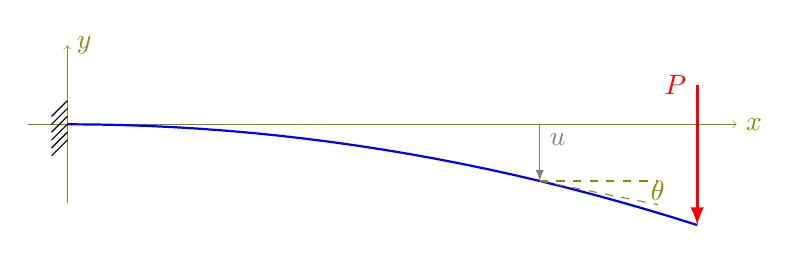
\begin{tikzpicture}[scale=1]
\draw  [very thin, olive] [->]  (-0.5,0) -- (8.5,0) node[right] {$x$};
\draw  [very thin, olive] [->]  (0,-1) -- (0,1) node[right] {$y$};
\draw [line width=2mm,blue,thick=6,domain=0:8] plot(\x,{-\x*\x/50});
%\draw  [line width=0.2mm, red] [->]  (8,0.5) -- (8,-1.28);
\draw[very thick,red,latex-] (8,-1.28)--(8,0.5) node[anchor=east]{$P$};
\draw[gray,latex-] (6,-0.72)--(6,0) node[below right]{$u$};
\draw[olive,dashed] (6,-0.72)--++(1.5,0) ;
\draw[olive,dashed] (6,-0.72)--++(1.5,-0.3) ;
\draw[olive] (7.5,-0.85) node{$\theta$};;

\pgfmathsetmacro{\y}{2}
\foreach \x in {-0.2,-0.1,...,0.3}{
\draw (0,\x) --++ (-0.2,-0.2);
}
\end{tikzpicture} 
\end{center}
On considère le problème de poutre en flexion et on admet que la flèche est solution de
\[EI_z\frac{\partial^4 u}{\partial x^4}=p(x)\]
où $I_z$ est le moment d'inertie de la section transversale par rapport à l'axe $z$ orthogonale au plan de flexion en son centre de gravité. $p(x)$ est la densité linéique des forces répartis . On admet aussi les conditions aux limites suivantes:
\[
F_0=\left.EI_z\frac{\partial^3 u}{\partial x^3}\right|_{x=0}\quad F_\ell=-\left.EI_z\frac{\partial^3 u}{\partial x^3}\right|_{x=\ell}\quad M_0=-\left.EI_z\frac{\partial^2 u}{\partial x^2}\right|_{x=0}\quad M_\ell=\left.EI_z\frac{\partial^2 u}{\partial x^2}\right|_{x=\ell}
\]

\begin{enumerate}
\item Montrer que la formulation variationnelle du problème s'écrit de la forme
\[
({\cal P}_v)\;\left\{
\begin{array}{l}
\mbox{Trouver } u\in V \mbox{ vérifiant}\\
a(u,v)=\ell(v)\quad \forall v\in V
\end{array}
\right.
\]

où \[ a(u,v)=\displaystyle EI_z\int_0^L\frac{\de^2 u}{dx^2}\cdot \frac{\de^2 v}{dx^2}\,\de x\]
et \[ \ell(v)=\displaystyle \int_0^L p\cdot v(x)\de x+F_0 \cdot v(0)+F_L \cdot v(L)+M_0 \cdot \frac{\partial v}{\partial x}(0)+M_L \cdot \frac{\partial v}{\partial x}(L)\]
\item le déplacement de la section transversale de la poutre supposée rigide est caractérisé par le vecteur \[U=\left(\begin{array}{c}
u\\\theta
\end{array} \right)\quad \mbox{ avec }\quad \theta=\displaystyle \frac{\de u}{\de x}\]

On fait alors un maillage régulier et en choisissant un élément fini de Hermite de type (1) qui utilise les déplacements et leur dérivées comme degrés de liberté ;
\begin{center}
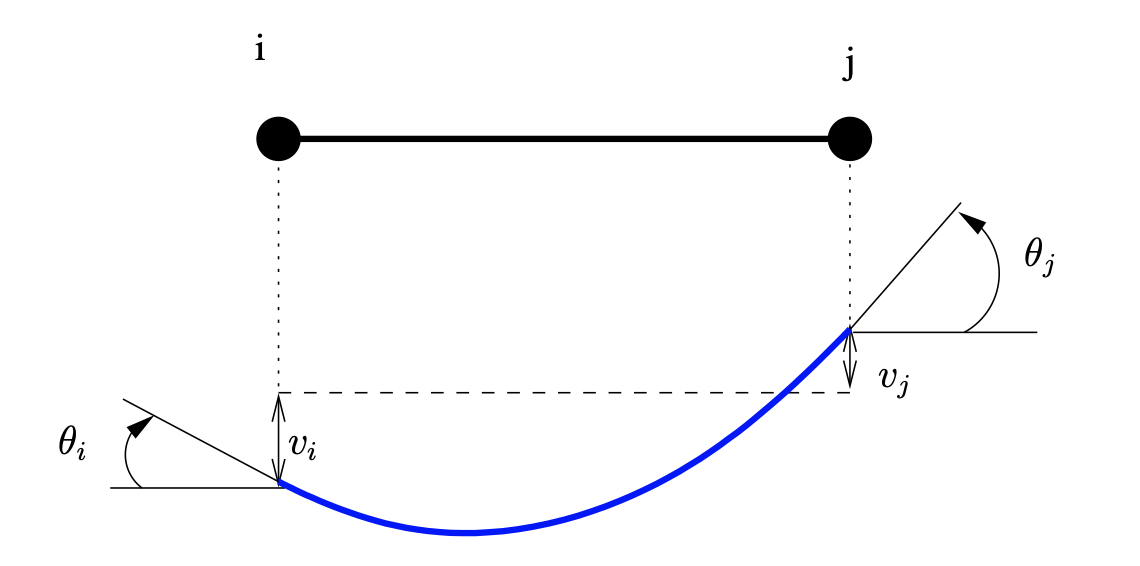
\includegraphics[scale=0.3]{poutreEnFlexion.png} 
\end{center}

 montrer que la matrice élémentaire s'écrit:
\[\frac{EI}{L^3}\left(\begin{array}{rrrr} 
12&6L&-12&6L\\
6L&4L^2&-6L&2L^2\\
-12&-6L&12&-6L\\
6L&2L^2&-6L&4L^2
\end{array}\right) 
\]

Déterminer le second membre élémentaire dans le cas où 
\begin{enumerate}
\item La poutre est bi-encastrée.
\item La poutre est encastrée à son origine et soumise à une force $\vec{P}$ à l'autre extrémité.
\end{enumerate}



\end{enumerate}
 
 
\end{document}





